%!TEX root = ../report.tex
\section{Divergence}
\label{sec:divergence}
Divergence shows how much fluid is sucked into a sink or pulled out of a source. 
Calculation of divergence is done by taking the derivatives of vector fields, which results in a scalar value.
Taking the derivative of a vector field can be done by using differences.
We decided to use the central difference in the $x$ - as well as in the $y$ direction, since this will yield the most stable outcome. 
The function will look like this:  $f:\mathbf{R}^2 \rightarrow \mathbf{R}^1$.
So once the divergence is computed, it is just a question of color mapping a scalar value as in section \ref{sec:color_mapping}.

Divergence at point $p_{x,y}$ can be calculated using a couple of steps:

\begin{equation*}
\begin{aligned}
\nabla d &= \Delta x + \Delta y \\
\Delta x &= p_{x+1,y} - p_{x-1,y} \\
\Delta y &= p_{x,y+1} - p_{x,y-1} \\
\end{aligned}
\end{equation*}

Divergence in action can be seen in figure \ref{fig:div_velo}.
\begin{figure}[htb]
    \centering
    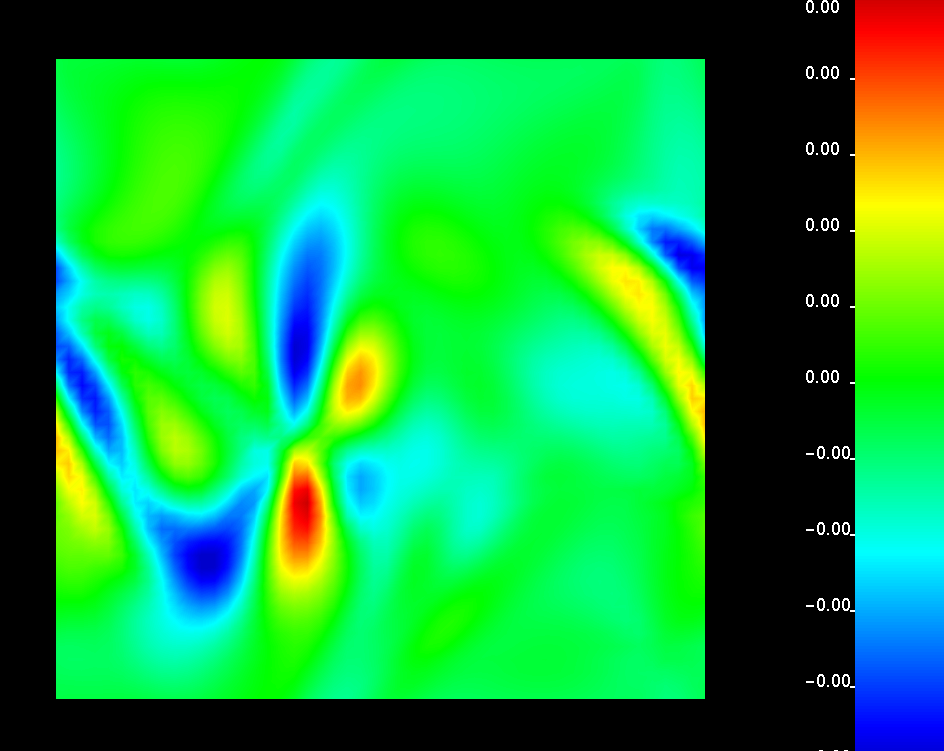
\includegraphics[width =0.5\textwidth]{content/pictures/div_velo.png}
    \caption{Divergence of the velocity field}
    \label{fig:div_velo}
\end{figure}

In figure \ref{fig:force_field} can be observed that there is a high correlation between the magnitude of the force field $||f||$ in figure \ref{fig:force_mag} and the divergence of this field $\nabla f$ in figure \ref{fig:div_force}.
The reason that these two visualizations are very similar is due to the simulation of the model, the model itself has no fixed sources or sinks. 
When the mouse is clicked, a source at that location is created, so sources exist on the locations where force is present.
\begin{figure}[htb]
    \centering
    \begin{subfigure}[htb]{.49\textwidth}
        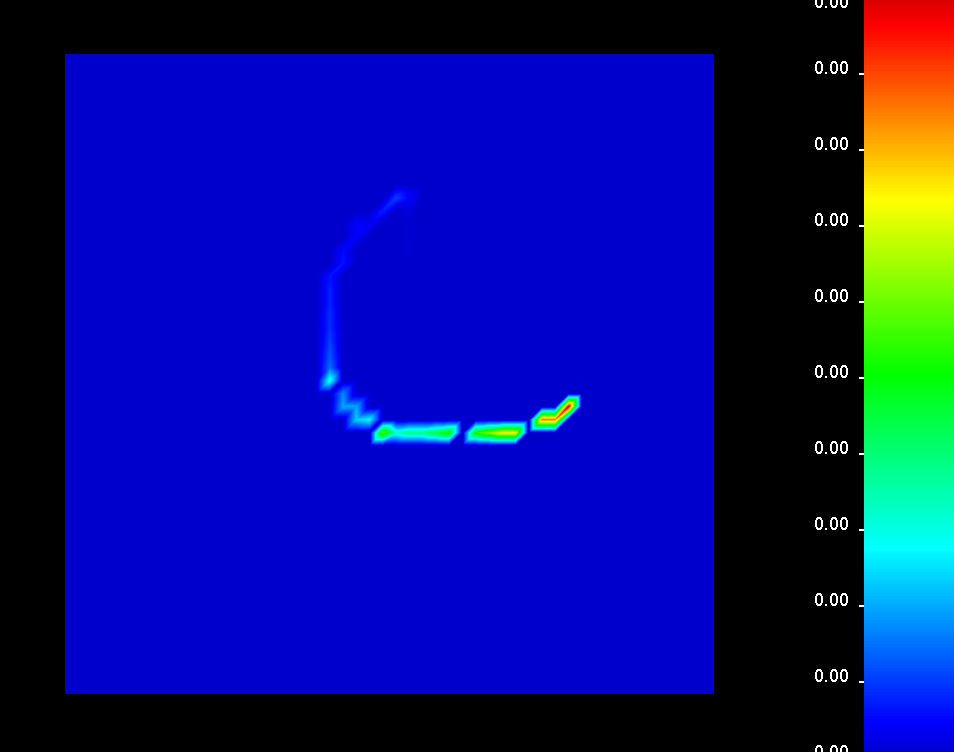
\includegraphics[width =\textwidth]{content/pictures/force_magnitude.png}
        \caption{Magnitude of force field ($||f||$)}
        \label{fig:force_mag}
    \end{subfigure}
    \begin{subfigure}[htb]{.49\textwidth}
        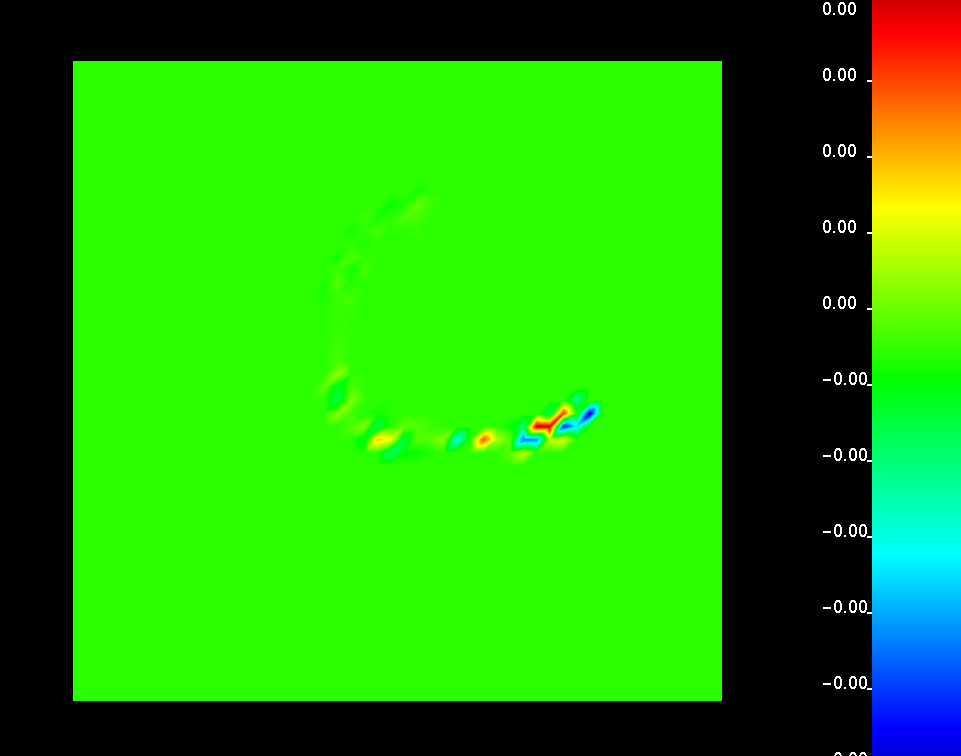
\includegraphics[width =\textwidth]{content/pictures/div_force.png}
        \caption{Divergence of force field ($\nabla f$) }
        \label{fig:div_force}
    \end{subfigure}
    \caption{Force field visualization}
    \label{fig:force_field}
\end{figure}


\clearpage